%----------------------------------------------------------------------------------------
%	PACKAGES AND THEMES
%----------------------------------------------------------------------------------------

\documentclass{beamer}

\mode<presentation> {

%\usetheme{default}
%\usetheme{AnnArbor}
%\usetheme{Antibes}
%\usetheme{Bergen}
%\usetheme{Berkeley}
%\usetheme{Berlin}
%\usetheme{Boadilla}
%\usetheme{CambridgeUS}
%\usetheme{Copenhagen}
%\usetheme{Darmstadt}
%\usetheme{Dresden}
%\usetheme{Frankfurt}
%\usetheme{Goettingen}
%\usetheme{Hannover}
\usetheme{Ilmenau}
%\usetheme{JuanLesPins}
%\usetheme{Luebeck}
%\usetheme{Madrid}
%\usetheme{Malmoe}
%\usetheme{Marburg}
%\usetheme{Montpellier}
%\usetheme{PaloAlto}
%\usetheme{Pittsburgh}
%\usetheme{Rochester}
%\usetheme{Singapore}
%\usetheme{Szeged}
%\usetheme{Warsaw}

% As well as themes, the Beamer class has a number of color themes
% for any slide theme. Uncomment each of these in turn to see how it
% changes the colors of your current slide theme.

%\usecolortheme{albatross}
\usecolortheme{beaver}			%JGU-mäßig
%\usecolortheme{beetle}
%\usecolortheme{crane}
%\usecolortheme{dolphin}		%Light blue
%\usecolortheme{dove}
%\usecolortheme{fly}
%\usecolortheme{lily}			%Dark blue
%\usecolortheme{orchid}
%\usecolortheme{rose}
%\usecolortheme{seagull}		%Grey
%\usecolortheme{seahorse}
%\usecolortheme{whale}
%\usecolortheme{wolverine}


\setbeamertemplate{navigation symbols}{} % To remove the navigation symbols from the bottom of all slides uncomment this line
}

\usepackage{graphicx}
\usepackage{booktabs}
\usepackage{multicol}
\usepackage[english]{babel}

%----------------------------------------------------------------------------------------
%	TITLE PAGE
%----------------------------------------------------------------------------------------

\title[CUDA-based Bruteforcing]{MD5 and SHA1 Bruteforcing using CUDA} % The short title appears at the bottom of every slide, the full title is only on the title page

\author{Oliver Gr\"ab} % Your name
\institute[JGU] % Your institution as it will appear on the bottom of every slide, may be shorthand to save space
{
Johannes Gutenberg University Mainz \\ % Your institution for the title page
\medskip
\textit{ograeb@students.uni-mainz.de} % Your email address
}
\date{April 15, 2016} % Date, can be changed to a custom date

\begin{document}

\begin{frame}
\titlepage% Print the title page as the first slide
\end{frame}

\begin{frame}
\frametitle{Overview} % Table of contents slide, comment this block out to remove it
\tableofcontents % Throughout your presentation, if you choose to use \section{} and \subsection{} commands, these will automatically be printed on this slide as an overview of your presentation
\end{frame}

%----------------------------------------------------------------------------------------
%	PRESENTATION SLIDES
%----------------------------------------------------------------------------------------

\section{About Hashing}

\begin{frame}
	\frametitle{General}
	\begin{block}{Hash Function}
		A hash function is any function that can be used to map data of arbitrary size to data of fixed size.
	\end{block}
	\begin{block}{Cryptographic Hash Function}
		A cryptographic hash function is a hash function which is considered practically impossible to invert
	\end{block}
	\footnotesize From \url{https://en.wikipedia.org/wiki/Hash_function}
\end{frame}

%------------------------------------------------

\begin{frame}
	\frametitle{MD5 message-digest algorithm}
	\begin{itemize}
		\item 128 bit Hash value
		\item RFC 1321 from 1992
		\item ``cryptographically broken and unsuitable for further use'' according to the CMU Software Engineering Institute
		\item Broken in $2^{18}$ time, less than a second
	\end{itemize}
\end{frame}

%------------------------------------------------

\begin{frame}
	\frametitle{SHA-1}
	\begin{itemize}
		\item 160 bit Hash value
		\item Designed by NIST in 1995
		\item ``No longer secure against well-funded opponents''
		\item Collision complexity $2^{60.3}-2^{65.3}$
		\item Replaced by SHA-2 and SHA-3
	\end{itemize}
\end{frame}

%------------------------------------------------

\section{Bruteforcing}

\begin{frame}
	\frametitle{Why Bruteforce?}
	Function not reversible

	$\Rightarrow$ Try all the inputs

	\vspace{1.5em}
	MD5:

	$2^{128}=340,282,366,920,938,463,463,374,607,431,768,211,456$ guesses

	\vspace{1em}
	SHA1: $2^{160}=1,461,501,637,330,902,918,203,684,832,716,283,019,655,932,542,976$ guesses

	\vspace{1.5em}
	That is why we need massive parallelism
\end{frame}

%------------------------------------------------
\begin{frame}
	\frametitle{Enumeration}
	\begin{center}
		How do we try everything?

		\vspace{1em}
		a\\
		b\\
		$\vdots$ \\
		Z\\
		aa\\
		ba\\
		$\vdots$

		\vspace{1em}
		Limit Inputs to $\{a-z, A-Z, 0-9\}$
	\end{center}
\end{frame}

%------------------------------------------------
\section{Implementation}

\begin{frame}
	\frametitle{Basic Implementation}
	\begin{enumerate}
		\item Get serial Implementation without global Variables
		\item Add CUDA annotations
		\item Feed with Strings
		\item ???????????
		\item PROFIT!
	\end{enumerate}
\end{frame}


%------------------------------------------------
\begin{frame}
	\frametitle{MD5}
	\begin{multicols}{2}
	[\centering Basic implementation is easy\\
	md5.cu]
		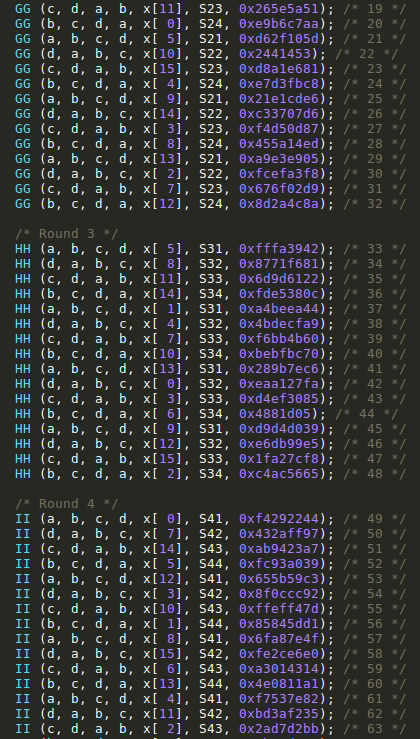
\includegraphics[height=.75\textheight]{md5_1.png}

		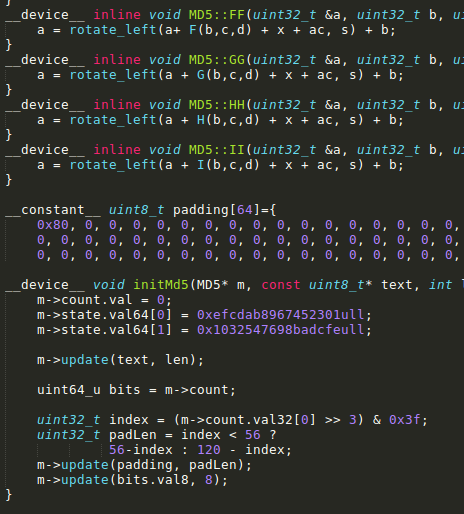
\includegraphics[height=.7\textheight]{md5_2.png}
	\end{multicols}
\end{frame}

%------------------------------------------------

\begin{frame}
	\frametitle{SHA1}
	\begin{multicols}{2}
	[\centering Basic implementation is easy\\
	SHA1.cu]
		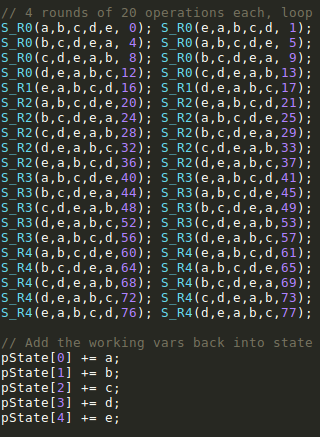
\includegraphics[height=.75\textheight]{sha1_1.png}

		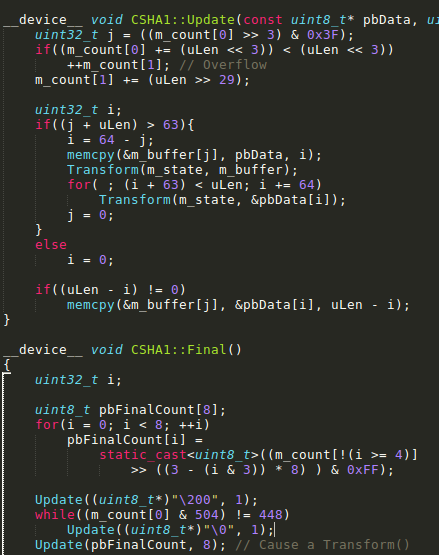
\includegraphics[height=.7\textheight]{sha1_2.png}
	\end{multicols}
\end{frame}

%------------------------------------------------

\begin{frame}
	\frametitle{Optimizations}
	\begin{itemize}
		\item{Shared Memory:}
			Crypto objects, current Strings, possible characters.

			48kB is plenty\dots
		\item{Constant Memory:}
			Hash which is searched (copied by host), padding for algorithm. Constants in general faster as literals.
		\item{Global Memory:}
			local Memory
	\end{itemize}

	\vspace{1em}
	Lots of bithacks

	Result: Not a single divergent branch

	\vspace{1em}
	Best runtime with 64 threads x 64 blocks
\end{frame}


%------------------------------------------------
\begin{frame}
	\frametitle{String enumeration}
	Using 64 symbols for simplicity: [a-z],[A-Z],[0-9],' ', '-'

	\begin{center}
		SHA1.cu / md5.cu

		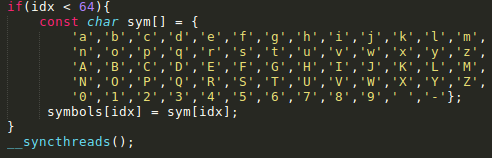
\includegraphics[width=.6\textwidth]{symbols.png}

		utility.cu

		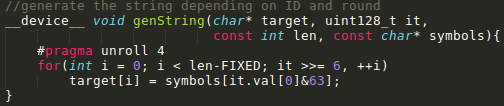
\includegraphics[width=.6\textwidth]{stringGeneration.png}
	\end{center}

	Fixed suffix depending on the global thread Id

	Needs $64^n$ total threads

\end{frame}

%------------------------------------------------

\begin{frame}
	\frametitle{128 Bit Integers}
	With more than 10 characters we need numbers larger than $2^{64}$ for the enumeration\dots
	\vspace{-1em}
	\begin{multicols}{2}[]
	\begin{center}
		bigInt.h

		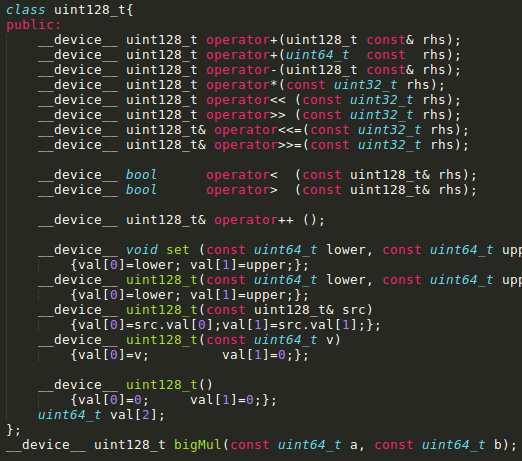
\includegraphics[width=.5\textwidth]{bigInt_1.png}

		bigInt.cu

		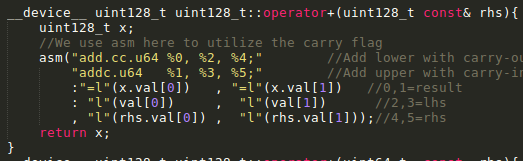
\includegraphics[width=.5\textwidth]{bigInt_2.png}

		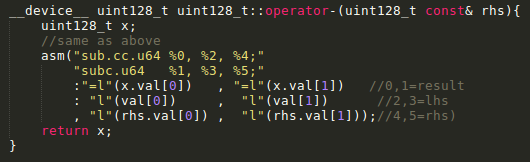
\includegraphics[width=.5\textwidth]{bigInt_3.png}

		Because assembly is FAST\@! (and can use the carry flag)
	\end{center}
	\end{multicols}
\end{frame}

%------------------------------------------------
\section{Performance}

\begin{frame}
	\frametitle{Multi-GPU?}
	Since the problem is embarrassingly parallel and I had some time left\dots

	\begin{center}
		md5.cu / SHA1.cu

		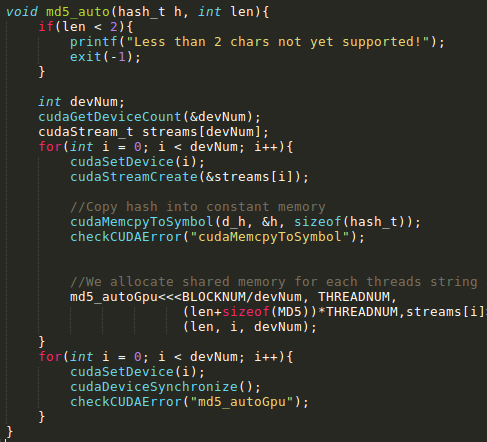
\includegraphics[width=.55\textwidth]{multiGpu.png}
	\end{center}

	Each Device gets 1/N of the search space (currently only for $2^n$ GPUs)
\end{frame}

%------------------------------------------------

\begin{frame}
	\frametitle{Performance of serial and parallel implementation}

	MD5, 4 characters

	i3--3110M @ 2.40GHz: 37.5 s

	GTX 480: 0.14 s

	\vspace{1em}
	Speedup around 270 on an older GPU

	\vspace{2em}
	Tests on GTX 680, 5 letters:

	MD5:  4.710s\\
	SHA1: 53.0s

	\vspace{1em}
	MD5:  228  MH/s
	SHA1: 20.3 MH/s
\end{frame}


%------------------------------------------------
\section{Demonstration}

\begin{frame}
	\frametitle{Demo!}
	\begin{center}
		GTX 480

		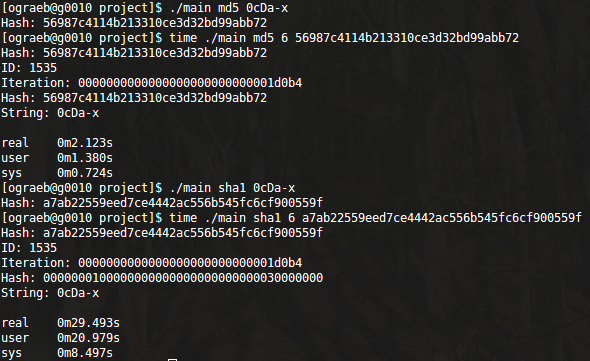
\includegraphics[width=.7\textwidth]{demo_1.png}
	\end{center}
	{\footnotesize Disregard wrong display in the picture}
\end{frame}

%------------------------------------------------
\section{Sources}

\begin{frame}
	\frametitle{Sources of Sample code etc.}
	\footnotesize{
	\begin{thebibliography}{99}
		\bibitem{wiki} Wikipedia
			\newblock{} Information about MD5, SHA1, Hash functions
			\newblock{} \url{https://en.wikipedia.org/wiki/}

		\bibitem{md5} MD5 implementation
			\newblock{} zedwood.com --- C++ MD5 function
			\newblock{} \url{http://www.zedwood.com/article/cpp-md5-function}

		\bibitem{sha1} SHA1 implementation
			\newblock{} Code Project --- CSHA1 - A C++ Class Implementation of the SHA-1 Hash Algorithm
			\newblock\url{http://www.codeproject.com/Articles/2463/CSHA-A-C-Class-Implementation-of-the-SHA-Hash-A}

		\bibitem{beamer} Latex Beamer template
			\newblock{} \LaTeX\ Templates --- Beamer Presentation
			\newblock{} \url{http://www.latextemplates.com/template/beamer-presentation}
	\end{thebibliography}
	}
\end{frame}

%------------------------------------------------

\begin{frame}
\Huge{\centerline{The End}}
\end{frame}

%----------------------------------------------------------------------------------------

\end{document}